%%%%%%%%%%%%%%%%%%%% author.tex %%%%%%%%%%%%%%%%%%%%%%%%%%%%%%%%%%%
%
% sample root file for your "contribution" to a proceedings volume
%
% Use this file as a template for your own input.
%
%%%%%%%%%%%%%%%% Springer %%%%%%%%%%%%%%%%%%%%%%%%%%%%%%%%%%


\documentclass{svproc}
%
% RECOMMENDED %%%%%%%%%%%%%%%%%%%%%%%%%%%%%%%%%%%%%%%%%%%%%%%%%%%
%

% to typeset URLs, URIs, and DOIs
\usepackage{url}

%I added in these packages manually
\def\UrlFont{\rmfamily}
\usepackage{natbib}%,bibspacing}
\usepackage{graphicx}
%\usepackage{subcaption}
\usepackage{bm}
%\usepackage{geometry}
\usepackage{float}
\usepackage{caption}
\usepackage{setspace}
\usepackage{amsmath}
\usepackage{multicol}
\usepackage{color}
\doublespacing
\usepackage[margin=1in]{geometry}


\def\UrlFont{\rmfamily}

\begin{document}
\mainmatter              % start of a contribution
%
\title{Expectation Maximization - Missing Data}
%
\titlerunning{Expectation Maximization}  % abbreviated title (for running head)
%                                     also used for the TOC unless
%                                     \toctitle is used
%
\author{Matthew Oehler}

\institute{Brigham Young University}
%
\authorrunning{Matt Oehler} % abbreviated author list (for running head)
%
%%%% list of authors for the TOC (use if author list has to be modified)

\maketitle              % typeset the title of the contribution

\begin{abstract}
Many parameter estimation techniques for multivariate distributions are not robust. They collapse in non-ideal cases, such as when dealing with a dataset that has missing values. In this study we explore three possible methods used to estimate parameters in the case of missing data. We will assess their overall performance through a Monte Carlo simulation study using multivariate normal distributed data, see how these methods can be used to find a pattern in the missing data, and then apply the methods to a dataset of the characteristics of hepatitis patients.
% We would like to encourage you to list your keywords within
% the abstract section using the \keywords{...} command.
\keywords{EM Algorithm, Parameter Estimation, Expectation-Maximization, Hepatitis}
\end{abstract}

%%%%%%%%%%%%%%%%%%%%%%%%%%%%%%%%%%%
\section{Introduction}
%
One of the fundamental focuses of statistics is to derive estimates of unknown population parameters. There are various ways to both theoretically and numerically derive estimates for parameters of multivariate distributions. Many of these methods, however, are not robust and fail when they encounter non-ideal circumstances, such as missing data. In this study we will look at three methods, including imputation methods, that can be uses to skirt the issues that arise when dealing with missing data. These methods are the throw-away method, the expectation-maximiation algorithm, and conditional sampling. These methods will be clearly defined and explored in more depth in following sections. The main questions we plan to answer through this study are as follows: Can we still derive good parameter estimates when there are missing data? And, Can we come up with a method to determine if the data are missing at random or if there is a pattern to the missingness? We performed a Monte Carlo simulation study using generated data that follows a multivariate normal distribution. We evaluated the performance of each method in cases where the data were randomly missing, and where the data were non-randomly missing. After assessing the performance of each method, we applied these three algorithms to a data set of characteristics of hepatitis patients. We chose to use this data set because it has missing values, and the data approximately follow a multivariate normal distribution. Other applications of the EM algorithm include data clustering, and latent variable analysis, but those topics will not be discussed in this paper.

%I originally intended to include a section about correlation estimates, but decided to omit it. 
%% And lastly, Can we determine which variables are most and least correlated? 

%%%%%%%%%%%%%%%%%%%%%%%%%%%%%%%%%
\section{Methodology}
%

\subsection{Throw-away Method}
The first method we assessed will be referred to as the throw-away method. It is important to note that this method doesn't have ubiquitous nomenclature, and it is informally refered to as the throw-away method throughout this study for the sake of consistency. It differs from the latter two methods in that it is actually not an imputation method. Rather this method estimates the parameters by removing all observations from the data set that are incomplete (i.e. by removing all observations where at least one of the dimensions is missing). The parameters are then estimated using the remaining data points (all of the complete observations). Since we focused on multivariate normal data, the multivariate normal probability density function and the appropraite estimates for the mean and variance-covariance matrix are shown below in equations \ref{eqpdf}, \ref{eq2}, and \ref{eq3} respectively.

\medskip
\textbf{MVN PDF:}
\begin{equation}
f(x|\mu,\Sigma) = \frac{1}{(2\pi)^{n/2}\vert \Sigma \vert^{1/2}} exp{ \bigl\{-\frac{1}{2}(x-\mu)^\top \Sigma^{-1}(x-\mu) \bigr\} }
\label{eqpdf}
\end{equation}




\textbf{Mean Estimate (MLE):}

\begin{equation}
\hat{\mu} = \frac{1}{N} \sum_{n=1}^N(x_n)
\label{eq2}
\end{equation}


\textbf{ Covariance Estimate (Unbiased): }
\begin{equation}
\hat{\Sigma} = \frac{1}{N-1} \sum_{n=1}^N(x_n - \bar{x})(x_n - \bar{x})^\top
\label{eq3}
\end{equation}


This is method can be appealing for a few reasons, especially under certain assumptions. First and foremost, this method is both easy to understand and easy to implement. Under the assumptions that the data are randomly missing and that the data is from a random sample this method is particularly appealing because even after throwing out many data points the estimates will still be unbiased. In essence, under those assumptions, the cost associated with removing values is identical to the cost of having a smaller sample when dealing with complete data. Some statisticians prefer this method over other more complex imputation methods becuase it can be argued that imputing data spreads the noise of the data throughout the entire dataset and artificially amplifies the effect of the present observations over the missing observations. The counter argument to the throw-away method is that removing observations when making estimates increases the uncertainty associated with those estimates. Also, in the case of the random missingness, and random sample assumptions not being met, estimates derived from the throw-away method are prone to higher error and bias. Despite having these down-sides, this method is commonly used in practice due to its simplicity.

\subsection{Expectation-Maximization Algorithm}

The second method we looked at is the expectation-maximization algorithm, commonly referred to as the EM algorithm. This method, rather than throwing out incomplete observations from the data set, keeps all observations and iteratively imputes appropriate means in the place of missing values until it converges. It uses the mean of the conditional multivariate normal distribution as the basis for its iterative updates. The conditional normal setup, and its parameters are shown in equations \ref{eqcond}, \ref{eq5}, and \ref{eq6} below.


%conditional normal setup
\begin{equation}
(\mathbf{x}_1 | \mathbf{x}_2=a) \sim N(\bar{\mu},\bar{\Sigma})
\label{eqcond}
\end{equation}

%conditional normal mean
\begin{equation}
\mathbf{\bar{\mu}} = \mathbf{\mu}_1 + \Sigma_{12}\Sigma_{22}^{-1}(a-\mu_{2})
\label{eq5}
\end{equation}

%conditional variance
\begin{equation}
\bar{\Sigma} = \Sigma_{11} - \Sigma_{12}\Sigma_{22}^{-1}\Sigma_{21}
\label{eq6}
\end{equation}

(Note: subscript 1 refers to missing values, and subscript 2 refers to non-missing values)


\medskip

The steps for the EM algorithm are as follows:
\begin{itemize}
\item (1) Set a tolerence level, $\epsilon$, at which the algorithm will converge.
\item (2) Set intial values for estimates of the mean vector $\mu$ and covariance matrix $\Sigma$.
(These estimates do not need to be accurate, the algorithm is fairly robust and will converge even with inaccurate starting values.)
\item (3) For every observation in the data set calculate and impute the mean from the conditional multivariate normal distribution. (This is the 'expectation' step).
\item (4) After all missing values have been imputed re-estimate the mean and covariance matrix using the formulas in equations \ref{eq2} and \ref{eq3}.
(This is the 'maximization' step.)
\item (5) Repeat steps 3 and 4 until the absolute difference between imputed matrices is less than the specified tolerance level, $\epsilon$. 
\item (6) Once the algorithm converges at the specified tolerance level, than the most recent estimates for the mean and covariance matrix are used as the overall parameter estimates. 
\end{itemize}

This method is appealing because it eliminates the need to get rid of information that is found in observations that are only partially collected. It also is suspected to perform better than the throw-away method in cases where the assumptions of randomness (in missing data, and sample gathering) are not met. Since the EM algorithm incorporates the variance in its imputation of the mean it is less susceptible to bias and error when the data are not missing at random. Due to its robustness, the EM algorithm is a strong alternative to the throw-away method. In the EM Algorithm Convergence Plot shown below in Figure \ref{convfig}, the robustness of the EM algorithm can be clearly seen. Even with inaccurate intial estimates, and a low tolerance, the algorithm converges quickly in under 40 iterations.

%%plot of convergence of EM algorithm
\begin{figure}

\begin{center}
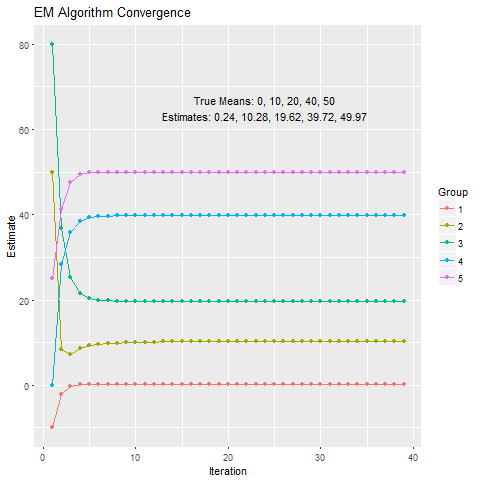
\includegraphics[width=0.65\linewidth]{EMconvergence-wonky}
\end{center}
\caption{Convergence of EM algorithm}
\label{convfig}
\end{figure}


\subsection{Conditional Sampling}
The third method we assessed will be referred to throughout this study as conditional sampling. This method, like the first, doesn't have a distinct name, but it is similar in design to the expectation-maximization algorithm while being slightly Bayesian in nature. Just like with the EM algorithm, conditional sampling iterates through each observation of the dataset, and imputes values using the conditional multivariate normal distribution. Unlike the EM algorithm, however, this method doesn't impute the mean of the conditional distribution. Instead, the conditional sampling method uses the iterative estimates of the mean vector and covariance matrix as parameters of the distribution from which we then take a random draw, and impute that value. After the all missing values have been imputed with random draws, the estimates for the mean and covariance are stored as draws, and the process is repeated many times. This algorithm is Bayesian in nature because it collects draws from a distribution and estimates the overall parameters based on the draws. Because it uses draws to estimate rather than imputed means, this algorithm does not converge. It will simply run for the pre-set number of iterations. Since this algorithm doesn't coverge, it also requires a pre-set number of burn-in samples, which are removed from the pool of draws before estimating and updating the parameters. The steps of this algorithm in detail are shown below.

Steps for conditional sampling:
\begin{itemize}
\item (1) Set the number of iterations for the algorithm to run, and a number of burn-in draws.
\item (2) Set the intial values for the estimates of the mean vector and covariance matrix.
\item (3) For every observation in the data set calculate mean vector and covariance matrix estimates for the missing values using the conditional multivariate normal distribution.
\item (4) Draw random values from a multivariate normal distribution using the estimates from step 3 as the parameters.
\item (5) After imputing all of the missing values, estimate the mean and covariance of the imputed data using the formulas in equations \ref{eq2} and \ref{eq3}.
\item (6) Store these new estimates in a list of the draws.
\item (7) Repeat steps 3-6 many times
\item (8) After removing the burn-in draws, estimate the overall mean vector and covariance matrix by taking the mean of each element across all draws, and use these as the overall estimates of the conditional sampling algorithm.
\end{itemize}

Conditional sampling is appealing similarly to the EM algorithm, because it doesn't involve removing any data from the dataset. It is also stronger than the throw-away method in cases where the data aren't missing at random, because it uses the covariance matrix in its estimation process. The flexibility of the conditional sampling method is also nice, because it can be explicity controlled to run for a set number of iterations. This provides the ability to adjust for how accurate the estimates need to be, and eliminates the need to wait for convergence (whereas the EM algorithm would take a long time) in complex cases.

%the math formulas and what not are already listed in the previous sections so I can just refer to them there
%make a note that this algorithm is bayesian in nature
%it doesnt converge
%it is cool that we can take as many or as little iterations as we deem necessary

\section{Simulation Study}
We performed a Monte Carlo simulation study to address the main research questions. We implemented all three methods on simulated data under the two cases of interset: when data are randomly missing, and when data are missing according to a pattern. We ran 10,000 MC iterations for each method, and we used a true mean vector of $\mu = [0,10,20,40,50]$ for data sets of 100 observations. We set the constant of .3 to be the proportion of the data that are missing for each iteration.  For this study, we looked only at the performance of the mean, but the estimates of the covariance can be assessed visually by plotting the fit of the parameter estimates for each method on the same graph. (There is a good example of this in the application section, where it will further be discussed.) For each method, and for each case we calculated the estimates, the estimate biases, and the mean squared error. The results for the case in which the data were randomly missing are shown in Table \ref{tab1}. 


%table of means for randomly missing data
\begin{table}[!ht]

\centering
\begin{tabular}{rrrr}
  \hline
Method & Estimate & Bias & MSE \\ 
  \hline
  Throw Away & 0.0010 & 0.0010 & 0.0621 \\ 
   & 10.0021 & 0.0021 & 0.0612 \\ 
   & 20.0023 & 0.0023 & 0.0615 \\ 
   & 40.0026 & 0.0026 & 0.0615 \\ 
   & 50.0034 & 0.0034 & 0.0620 \\   \hline
  EM Algorithm & 0.0008 & 0.0008 & 0.0124 \\ 
   & 10.0049 & 0.0049 & 0.0135 \\ 
   & 20.0048 & 0.0048 & 0.0139 \\ 
   & 40.0022 & 0.0022 & 0.0125 \\ 
   & 50.0027 & 0.0027 & 0.0144 \\   \hline
  Conditional Sampling & -0.0062 & -0.0062 & 0.0122 \\ 
   & 9.9961 & -0.0039 & 0.0126 \\ 
   & 19.9973 & -0.0027 & 0.0142 \\ 
   & 39.9920 & -0.0080 & 0.0118 \\ 
   & 49.9990 & -0.0010 & 0.0157 \\ 
   \hline
\end{tabular}

\caption{Estimates for mean vector based on data with randomly removed values.}
\label{tab1}
\end{table}

We can see that the estimates are all accurate and unbiased to at least two decimal places away from the true value. The main take away from this first case study is that the MSE for the throw-away method is significanly higher for all values than both the EM algorithm and conditional sampling methods. This makes sense because the throw-away method makes these estimates using less information, so the error is naturally going to be higher. 
%talk about how I used random and non random missing data to look for a pattern

%table for nonrandomly missing data

The MC simulation conditions for the second case (non-random missing data) were identical to the conditions of the first case, except instead of randomly allocated missing values, we chose to eliminate all values that were greater than 1.5 standard deviations above the mean. We chose to impose this constraint because there are several real-world applications in which measuring techniques can't exceed a certain point. Sometime these data points are recorded as the maximum value, but other times they are left out altogether. There are many other realistic constraints that can be imposed, (and they would likely yeild new insights and/or conclusions) but for this study we only imposed this one restraint. The results of the second case, in which the data were non-randomly missing, are shown in Table \ref{tab2}.

\begin{table}[!!!!h]

\centering
\begin{tabular}{rrrr}
  \hline
 & Estimate & Bias & MSE \\ 
  \hline
  Throw Away & -0.2541 & -0.2541 & 0.0725 \\ 
   & 9.7889 & -0.2111 & 0.0527 \\ 
   & 19.7803 & -0.2197 & 0.0566 \\ 
   & 39.7524 & -0.2476 & 0.0689 \\ 
   & 49.7926 & -0.2074 & 0.0514 \\ \hline
  EM Algorithm & -0.0931 & -0.0931 & 0.0172 \\ 
   & 9.8625 & -0.1375 & 0.0234 \\ 
   & 19.8898 & -0.1102 & 0.0162 \\ 
   & 39.8926 & -0.1074 & 0.0154 \\ 
   & 49.8481 & -0.1519 & 0.0307 \\ \hline
  Conditional Sampling & -0.0871 & -0.0871 & 0.0155 \\ 
   & 9.9055 & -0.0945 & 0.0165 \\ 
   & 19.8943 & -0.1057 & 0.0188 \\ 
   & 39.9142 & -0.0858 & 0.0150 \\ 
   & 49.8757 & -0.1243 & 0.0229 \\ 
   \hline
\end{tabular}
\caption{Estimates for mean vector based on data where any value greater than 1.5 standard deviations above the mean were removed.}
\label{tab2}
\end{table}

We can see that for the case of non-random missing data, the mean vector estimates for all 3 methods are negatively biased. This is expected since we removed only values from the higher extreme of the distribution. It is also interesting to note that the MSE for the throw-away method stayed about the same on average, but that the MSE for both the EM algorithm and conditional sampling increased. We can also see that the mean estimates for the throw away method are more biased than the estimates of the EM algorithm and conditional sampling. The EM algorithm and conditional sampling method performed almost identically, while the throw-away method estimates differed. This result shows us that we can indeed use these methods to find a pattern in the missingness of the data. We can identify that there is a pattern by looking at the difference of the throw-away method estimates compared to the EM algorithm and/or conditional sampling estimates. In this case the difference isn't enormous and so we can't provide super solid conclusions as to the strength or existence of the pattern, but further studies that test the results under different conditions (number of iterations, percent of data that are missing, etc) and contraints (rules to dictate how the data is missing for the second case), could possibly show ways to optimize comparisons to best detect patterns of data-missingness. The goal of this study was simply to see if a pattern can be detected. 

Another, more solid, conclusion that can be drawn from both cases addresses the first research question: Can we still get good parameter estimates in the presence of missing data. Both cases of the simulation study show that these three different methods yield quite accurate results.  It is also important to note that these are just three of many possible methods of dealing with missing data. Other methods could also be explored and could potentially provide more accurate estimates. 

\section{Application and Results}

Next we used the three methods discussed above were applied to a data set of characteristics of hepatitis patients. In practice, this data set would best be utilized to potentially model the traits of patients that prove useful in predicting whether a patient has, or is likely to contract hepatitis. For this study, however, we will simply use it to compare the performance of the throw-away method, the EM algorithm, and conditional sampling. We chose this data set because it has many missing values, and it is assumed to follow a multivariate normal distribution. Since the three methods we are testing only apply to quantitative data, we removed all of the categorical data before hand. The remaining variables are: Age, Bilirubin, Alkaline Phospate (AlkPhosphate), SGOT, Albumin, and Prothrombin Time (ProTime). Bilirubin refers to the amount of bilirubin in one's blood (it can be indicitive of conditions like jaundice and anemia). The remaining variables (Alkaline Phosphate, SGOT, Albumin and Prothrombin Time) are all different measures of liver function. A snippet of the data set is shown in Table \ref{tab3} .

After running all three methods, we ended up with the results that are displayed in Table \ref{tab4}. Based on the values in the table we can see that all the methods performed in the same ball park as each other, helps to to confirm that our estimates are good. Then, using the result of our simulation study, it looks like there might be a pattern of data missingness for the AlkPhospate and Bilirubin variables. The difference in the means, per scale of the variable, is the greatest for the estimates of those two variables when comparing the throw-away method to the other two methods. Figure \ref{fig1} shows how well the estimated parameters for each of the methods fit the data. From this figure we can see again that the EM Algorithm and conditional sampling perform almost identically. We can also see that the goodness of fit depends on how true the normality assumption actually is, since the fit isn't very good for the variables that aren't normally distributed (e.g. Sgot). Figure \ref{fig1} is also the best visual aid to compare the covariance estimates between the methods. 

%table of data head
\begin{table}[!h]
\centering
\begin{tabular}{rrrrrrr}
  \hline
  Age & Bilirubin & AlkPhosphate & Sgot & AlbuMin & ProTime \\ 
  \hline
    30 & 1.00 &  85 &  18 & 4.00 &  \\ 
    50 & 0.90 & 135 &  42 & 3.50 &  \\ 
    78 & 0.70 &  96 &  32 & 4.00 &  \\ 
    31 & 0.70 &  46 &  52 & 4.00 &  80 \\ 
    34 & 1.00 &  & 200 & 4.00 &  \\ 
    34 & 0.90 &  95 &  28 & 4.00 &  75 \\ 
   \hline
\end{tabular}
\caption{Snippet of the hepatitis data set}
\label{tab3}
\end{table}

%table of hep data estimates for mean for each method
\begin{table}[h]
\centering
\begin{tabular}{rrrr}
  \hline
 & Throw Away & EM Algorithm & Conditional Sampling \\ 
  \hline
Age & 41.06 & 41.20 & 41.20 \\ 
  Bilirubin & 1.25 & 1.43 & 1.43 \\ 
  AlkPhosphate & 102.51 & 106.30 & 106.31 \\ 
  Sgot & 86.39 & 85.89 & 85.92 \\ 
  AlbuMin & 3.83 & 3.81 & 3.81 \\ 
  ProTime & 62.16 & 61.81 & 61.74 \\ 
   \hline
\end{tabular}

\caption{Estimates from each method for the hepatitis data set}
\label{tab4}
\end{table}


%%the super gorgeous goodness of fit graph that is my baby
\begin{figure}[!h]
\begin{center}
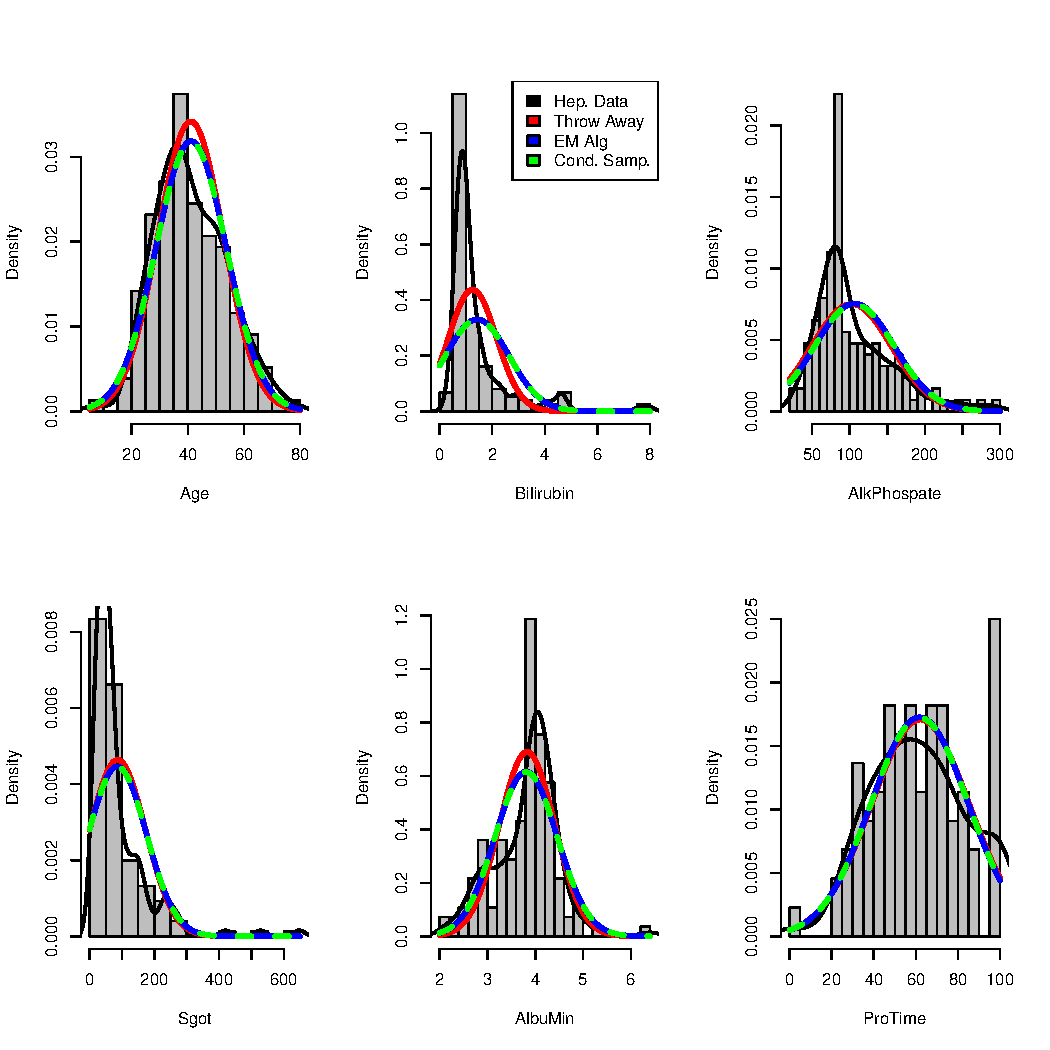
\includegraphics[width=0.65\linewidth]{goodnessoffit}
\end{center}
\caption{Fit of parameter estimates to the data for each method}
\label{fig1}
\end{figure}

\pagebreak

\section{Conclusions}
Overall, we were able to address several things in this study. We showed that even when dealing with missing data it is still possible to get good parameter estimates. We also showed that if the throw-away method estimates differ from the EM algorithm and conditional sampling estimates, we can conclude that there is a pattern to the missingness of the data. Then by applying these methods to the hepatitis data set, we showed how well the algorithms perform in comparison to each other, and that they perform best on data that truly follows a normal distribution.This study though, could still be augmented in several ways. There is still much to explore concerning the methods of detecting patterns in missing data, trying different constraints for the non-randomly missing case study, and assessing the confidence of the conclusions that we can draw using these methods. It would also be interesting to see which imputation methods are best at enhancing the prediction accuracy of hepatitis patients for various modeling methods that are based on the hepatitis data that we used for this study, or to look at how the estimates of covariance matrix can be used to assess the correlation between variables. Even though there is more that could to be done, through this study we were successfully able to explore the details of the throw-away method, the EM algorithm, and conditional sampling, and we answered the research questions that we started with. 

%\section{Appendix}





%%%%%%%  GARBAGE %%%%%%%%%%%%%%%%%%%%%%%%%%%%%%%%%%%%%%%%%%%%%%%%%%
%


%We recall once more that by the integer part $E [\alpha ]$ of
%$\alpha \in \bbbr$, we mean the $a\in \bbbz$
%such that $a< \alpha \le a+1$. For instance,
%if we take $a_{\infty} = 0$, Corollary 2 tells
%us that $\overline{x}$ exists and is
%non-constant provided that:
%
%\begin{equation}
%  \frac{T}{2\pi} b_{\infty} < 1 < \frac{T}{2\pi}
%\end{equation}
%or
%\begin{equation}
%  T\in \left(\frac{2\pi}{\omega},\frac{2\pi}{b_{\infty}}\right)\ .
%  \label{eq:four}
%\end{equation}
%
%%
%\begin{proof}
%The spectrum of $\Lambda$ is $\frac{2\pi}{T} \bbbz +a_{\infty}$. The
%largest negative eigenvalue $\lambda$ is given by
%$\frac{2\pi}{T}k_{o} +a_{\infty}$,
%where
%\begin{equation}
%  \frac{2\pi}{T}k_{o} + a_{\infty} < 0
%  \le \frac{2\pi}{T} (k_{o} +1) + a_{\infty}\ .
%\end{equation}
%Hence:
%\begin{equation}
%  k_{o} = E \left[- \frac{T}{2\pi} a_{\infty}\right] \ .
%\end{equation}
%
%The condition $\gamma < -\lambda < \delta$ now becomes:
%\begin{equation}
%  b_{\infty} - a_{\infty} <
%  - \frac{2\pi}{T} k_{o} -a_{\infty} < \omega -a_{\infty}
%\end{equation}
%which is precisely condition (\ref{eq:three}).\qed
%\end{proof}
%%
%
%\begin{lemma}
%Assume that $H$ is $C^{2}$ on $\bbbr^{2n} \setminus \{ 0\}$ and
%that $H'' (x)$ is non-de\-gen\-er\-ate for any $x\ne 0$. Then any local
%minimizer $\widetilde{x}$ of $\psi$ has minimal period $T$.
%\end{lemma}
%%
%\begin{proof}
%We know that $\widetilde{x}$, or
%$\widetilde{x} + \xi$ for some constant $\xi
%\in \bbbr^{2n}$, is a $T$-periodic solution of the Hamiltonian system:
%\begin{equation}
%  \dot{x} = JH' (x)\ .
%\end{equation}
%
%There is no loss of generality in taking $\xi = 0$. So
%$\psi (x) \ge \psi (\widetilde{x} )$
%for all $\widetilde{x}$ in some neighbourhood of $x$ in
%$W^{1,2} \left(\bbbr / T\bbbz ; \bbbr^{2n}\right)$.
%
%But this index is precisely the index
%$i_{T} (\widetilde{x} )$ of the $T$-periodic
%solution $\widetilde{x}$ over the interval
%$(0,T)$, as defined in Sect.~2.6. So
%\begin{equation}
%  i_{T} (\widetilde{x} ) = 0\ .
%  \label{eq:five}
%\end{equation}
%
%Now if $\widetilde{x}$ has a lower period, $T/k$ say,
%we would have, by Corollary 31:
%\begin{equation}
%  i_{T} (\widetilde{x} ) =
%  i_{kT/k}(\widetilde{x} ) \ge
%  ki_{T/k} (\widetilde{x} ) + k-1 \ge k-1 \ge 1\ .
%\end{equation}
%
%This would contradict (\ref{eq:five}), and thus cannot happen.\qed
%\end{proof}
%\section{Literature Review}
%Maybe
%\section{Methodology}
%You choose
%
%\section{Results}
%Loots of thing can go here
%%
%\paragraph{Notes and Comments.}
%The results in this section are a
%refined version of \cite{smit:wat};
%the minimality result of Proposition
%14 was the first of its kind.
%
%To understand the nontriviality conditions, such as the one in formula
%(\ref{eq:four}), one may think of a one-parameter family
%$x_{T}$, $T\in \left(2\pi\omega^{-1}, 2\pi b_{\infty}^{-1}\right)$
%of periodic solutions, $x_{T} (0) = x_{T} (T)$,
%with $x_{T}$ going away to infinity when $T\to 2\pi \omega^{-1}$,
%which is the period of the linearized system at 0.
%
%\begin{table}
%\caption{This is the example table taken out of {\it The
%\TeX{}book,} p.\,246}
%\begin{center}
%\begin{tabular}{r@{\quad}rl}
%\hline
%\multicolumn{1}{l}{\rule{0pt}{12pt}
%                   Year}&\multicolumn{2}{l}{World population}\\[2pt]
%\hline\rule{0pt}{12pt}
%8000 B.C.  &     5,000,000& \\
%  50 A.D.  &   200,000,000& \\
%1650 A.D.  &   500,000,000& \\
%1945 A.D.  & 2,300,000,000& \\
%1980 A.D.  & 4,400,000,000& \\[2pt]
%\hline
%\end{tabular}
%\end{center}
%\end{table}
%%
%\begin{theorem} [Ghoussoub-Preiss]\label{ghou:pre}
%Assume $H(t,x)$ is
%$(0,\varepsilon )$-subquadratic at
%infinity for all $\varepsilon > 0$, and $T$-periodic in $t$
%\begin{equation}
%  H (t,\cdot )\ \ \ \ \ {\rm is\ convex}\ \ \forall t
%\end{equation}
%\begin{equation}
%  H (\cdot ,x)\ \ \ \ \ {\rm is}\ \ T{\rm -periodic}\ \ \forall x
%\end{equation}
%\begin{equation}
%  H (t,x)\ge n\left(\left\|x\right\|\right)\ \ \ \ \
%  {\rm with}\ \ n (s)s^{-1}\to \infty\ \ {\rm as}\ \ s\to \infty
%\end{equation}
%\begin{equation}
%  \forall \varepsilon > 0\ ,\ \ \ \exists c\ :\
%  H(t,x) \le \frac{\varepsilon}{2}\left\|x\right\|^{2} + c\ .
%\end{equation}
%
%Assume also that $H$ is $C^{2}$, and $H'' (t,x)$ is positive definite
%everywhere. Then there is a sequence $x_{k}$, $k\in \bbbn$, of
%$kT$-periodic solutions of the system
%\begin{equation}
%  \dot{x} = JH' (t,x)
%\end{equation}
%such that, for every $k\in \bbbn$, there is some $p_{o}\in\bbbn$ with:
%\begin{equation}
%  p\ge p_{o}\Rightarrow x_{pk} \ne x_{k}\ .
%\end{equation}
%\qed
%\end{theorem}
%%
%\begin{example} [{{\rm External forcing}}]
%Consider the system:
%\begin{equation}
%  \dot{x} = JH' (x) + f(t)
%\end{equation}
%where the Hamiltonian $H$ is
%$\left(0,b_{\infty}\right)$-subquadratic, and the
%forcing term is a distribution on the circle:
%\begin{equation}
%  f = \frac{d}{dt} F + f_{o}\ \ \ \ \
%  {\rm with}\ \ F\in L^{2} \left(\bbbr / T\bbbz; \bbbr^{2n}\right)\ ,
%\end{equation}
%where $f_{o} : = T^{-1}\int_{o}^{T} f (t) dt$. For instance,
%\begin{equation}
%  f (t) = \sum_{k\in \bbbn} \delta_{k} \xi\ ,
%\end{equation}
%where $\delta_{k}$ is the Dirac mass at $t= k$ and
%$\xi \in \bbbr^{2n}$ is a
%constant, fits the prescription. This means that the system
%$\dot{x} = JH' (x)$ is being excited by a
%series of identical shocks at interval $T$.
%\end{example}
%%
%\begin{definition}
%Let $A_{\infty} (t)$ and $B_{\infty} (t)$ be symmetric
%operators in $\bbbr^{2n}$, depending continuously on
%$t\in [0,T]$, such that
%$A_{\infty} (t) \le B_{\infty} (t)$ for all $t$.
%
%A Borelian function
%$H: [0,T]\times \bbbr^{2n} \to \bbbr$
%is called
%$\left(A_{\infty} ,B_{\infty}\right)$-{\it subquadratic at infinity}
%if there exists a function $N(t,x)$ such that:
%\begin{equation}
%  H (t,x) = \frac{1}{2} \left(A_{\infty} (t) x,x\right) + N(t,x)
%\end{equation}
%\begin{equation}
%  \forall t\ ,\ \ \ N(t,x)\ \ \ \ \
%  {\rm is\ convex\ with\  respect\  to}\ \ x
%\end{equation}
%\begin{equation}
%  N(t,x) \ge n\left(\left\|x\right\|\right)\ \ \ \ \
%  {\rm with}\ \ n(s)s^{-1}\to +\infty\ \ {\rm as}\ \ s\to +\infty
%\end{equation}
%\begin{equation}
%  \exists c\in \bbbr\ :\ \ \ H (t,x) \le
%  \frac{1}{2} \left(B_{\infty} (t) x,x\right) + c\ \ \ \forall x\ .
%\end{equation}
%
%If $A_{\infty} (t) = a_{\infty} I$ and
%$B_{\infty} (t) = b_{\infty} I$, with
%$a_{\infty} \le b_{\infty} \in \bbbr$,
%we shall say that $H$ is
%$\left(a_{\infty},b_{\infty}\right)$-subquadratic
%at infinity. As an example, the function
%$\left\|x\right\|^{\alpha}$, with
%$1\le \alpha < 2$, is $(0,\varepsilon )$-subquadratic at infinity
%for every $\varepsilon > 0$. Similarly, the Hamiltonian
%\begin{equation}
%H (t,x) = \frac{1}{2} k \left\|k\right\|^{2} +\left\|x\right\|^{\alpha}
%\end{equation}
%is $(k,k+\varepsilon )$-subquadratic for every $\varepsilon > 0$.
%Note that, if $k<0$, it is not convex.
%\end{definition}
%%
%\section{Summary and Conclusions}  What do you want
%\paragraph{Notes and Comments.}
%The first results on subharmonics were
%obtained by Rabinowitz in \cite{fo:kes:nic:tue}, who showed the existence of
%infinitely many subharmonics both in the subquadratic and superquadratic
%case, with suitable growth conditions on $H'$. Again the duality
%approach enabled Clarke and Ekeland in \cite{may:ehr:stein} to treat the
%same problem in the convex-subquadratic case, with growth conditions on
%$H$ only.
%
%Recently, Michalek and Tarantello (see \cite{fost:kes} and \cite{czaj:fitz})
%have obtained lower bound on the number of subharmonics of period $kT$,
%based on symmetry considerations and on pinching estimates, as in
%Sect.~5.2 of this article.

%%
%% ---- Bibliography ----
%%
%\begin{thebibliography}{6}
%%
%
%\bibitem {smit:wat}
%Smith, T.F., Waterman, M.S.: Identification of common molecular subsequences.
%J. Mol. Biol. 147, 195?197 (1981). \url{doi:10.1016/0022-2836(81)90087-5}
%
%\bibitem {may:ehr:stein}
%May, P., Ehrlich, H.-C., Steinke, T.: ZIB structure prediction pipeline:
%composing a complex biological workflow through web services.
%In: Nagel, W.E., Walter, W.V., Lehner, W. (eds.) Euro-Par 2006.
%LNCS, vol. 4128, pp. 1148?1158. Springer, Heidelberg (2006).
%\url{doi:10.1007/11823285_121}
%
%\bibitem {fost:kes}
%Foster, I., Kesselman, C.: The Grid: Blueprint for a New Computing Infrastructure.
%Morgan Kaufmann, San Francisco (1999)
%
%\bibitem {czaj:fitz}
%Czajkowski, K., Fitzgerald, S., Foster, I., Kesselman, C.: Grid information services
%for distributed resource sharing. In: 10th IEEE International Symposium
%on High Performance Distributed Computing, pp. 181?184. IEEE Press, New York (2001).
%\url{doi: 10.1109/HPDC.2001.945188}
%
%\bibitem {fo:kes:nic:tue}
%Foster, I., Kesselman, C., Nick, J., Tuecke, S.: The physiology of the grid: an open grid services architecture for distributed systems integration. Technical report, Global Grid
%Forum (2002)
%
%\bibitem {onlyurl}
%National Center for Biotechnology Information. \url{http://www.ncbi.nlm.nih.gov}
%%%%%%%%  GARBAGE %%%%%%%%%%%%%%%%%%%%%%%%%%%%%%%%%%%%%%%%%%%
%
%
%
%\end{thebibliography}

\end{document}
